\input ../SlidePreamble
\input ../preamble

\begin{document}

{\Huge

  \centerline{\bf TTIC 31230, Fundamentals of Deep Learning}
  \bigskip
  \centerline{David McAllester, Winter 2020}

  \vfill
  \centerline{\bf AlphaStar}
  \vfill
  \vfill

  \slide{AlphaStar}

Grandmaster level in StarCraft II using multi-agent reinforcement learning, Nature Oct. 2019, Vinyals et al.

\vfill
StarCraft:

\begin{itemize}
\item Players control hundreds of units.

\vfill
\item Individual actions are selected from $10^{26}$ possibilities (an action is a kind of procedure call with arguments).

\vfill
\item Cyclic non-transitive strategies (rock-paper-scisors).

\vfill
\item Imperfect information --- the state is not fully observable.
\end{itemize}

\slide{The Paper is Vague}

It basically says the following ideas are used:

A policy gradient algorithm, auto-regressive policies, self-attention over the observation history, LSTMs, pointer-networks, scatter connections,
replay buffers, asynchronous advantage actor-critic algorithms, TD($\lambda$) (gradients on value function Bellman error), clipped importance sampling
(V-trace), a new undefined method they call UPGO that ``moves policies toward trajectories with better than average reward'', a value function
that can see the opponents observation (training only), a ``$z$ statistic'' stating a high level strategy, 
supervised learning from human play, 
a ``league'' of players (next slide).

\slide{The League}

The league has three classes of agents: main (M), main exploiters (E), and league exploiters (L).  M and L play against everybody.
E plays only against M.

\slide{A Rube Goldberg Contraption?}

\centerline{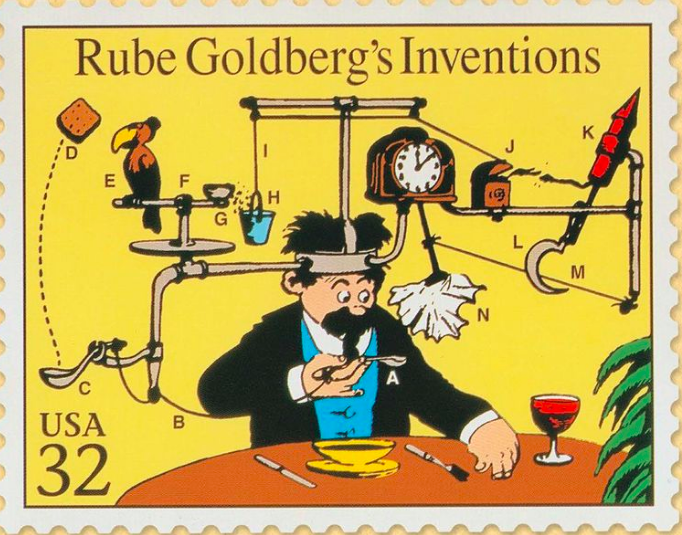
\includegraphics[height = 5in]{\images/Goldberg}}

\slide{Video}

https://www.youtube.com/watch?v=UuhECwm31dM

\slide{END}



}
\end{document}
